\chapter{Bestimmung der IQE bei Raumtemperatur}

\label{chap:raum}
\thispagestyle{fancy}

In diesem Kapitel wird die in Kapitel \ref{chap:grundfitting} vorgestellte Methode zur Bestimmung der IQE bei Raumtemperatur benutzt und versucht auf eine möglichst große Anzahl von uns gemessenen Proben anzuwenden. 
\newline
Um dies generisch und automatisiert zu verwirklichen und die Methode auf möglichst viele und auch alte Messungen anzuwenden, wurde von mir ein Mathematica-Skript geschrieben, dass die gemessenen Daten einer Probenserie bei Raumtemperatur benutzt, um die Ergebnisse in Echtzeit in Abhängigkeit von einem variablen Bereich der Messpunkte darzustellen. Dies erscheint wichtig, weil die Methode das ABC-Modell auf die Parameter A und B reduziert und somit möglichst ein Bereich ausgewählt werden sollte, bei dem der Einfluss der Auger-Rekombination gering ausfällt. Also muss insbesondere der Bereich geringer Anregungsleistungsdichten betrachtet werden, der allerdings mit unserem UVPL-Setup stark von Messartefakten und Rauschen beeinflusst ist.
\newline
Für die Anwendung der Methode wurden die Werte für die Fresnel-Reflexion $R$ variiert im Bereich von 
$0.1$ bis $0.9$ und für den Absorptionskoeffizienten $\alpha$ im Bereich $1\cdot 10^4$ bis $1\cdot 10^7 \thinspace \frac{1}{cm}$. Es zeigte sich, dass die Variation der Parameter nur einen Einfluss auf die die Generationsrate hat, allerdings nicht auf die resultierende IQE die unter der Variation konstant blieb. 
\begin{figure}[H]
\begin{tabular}{ccc}
  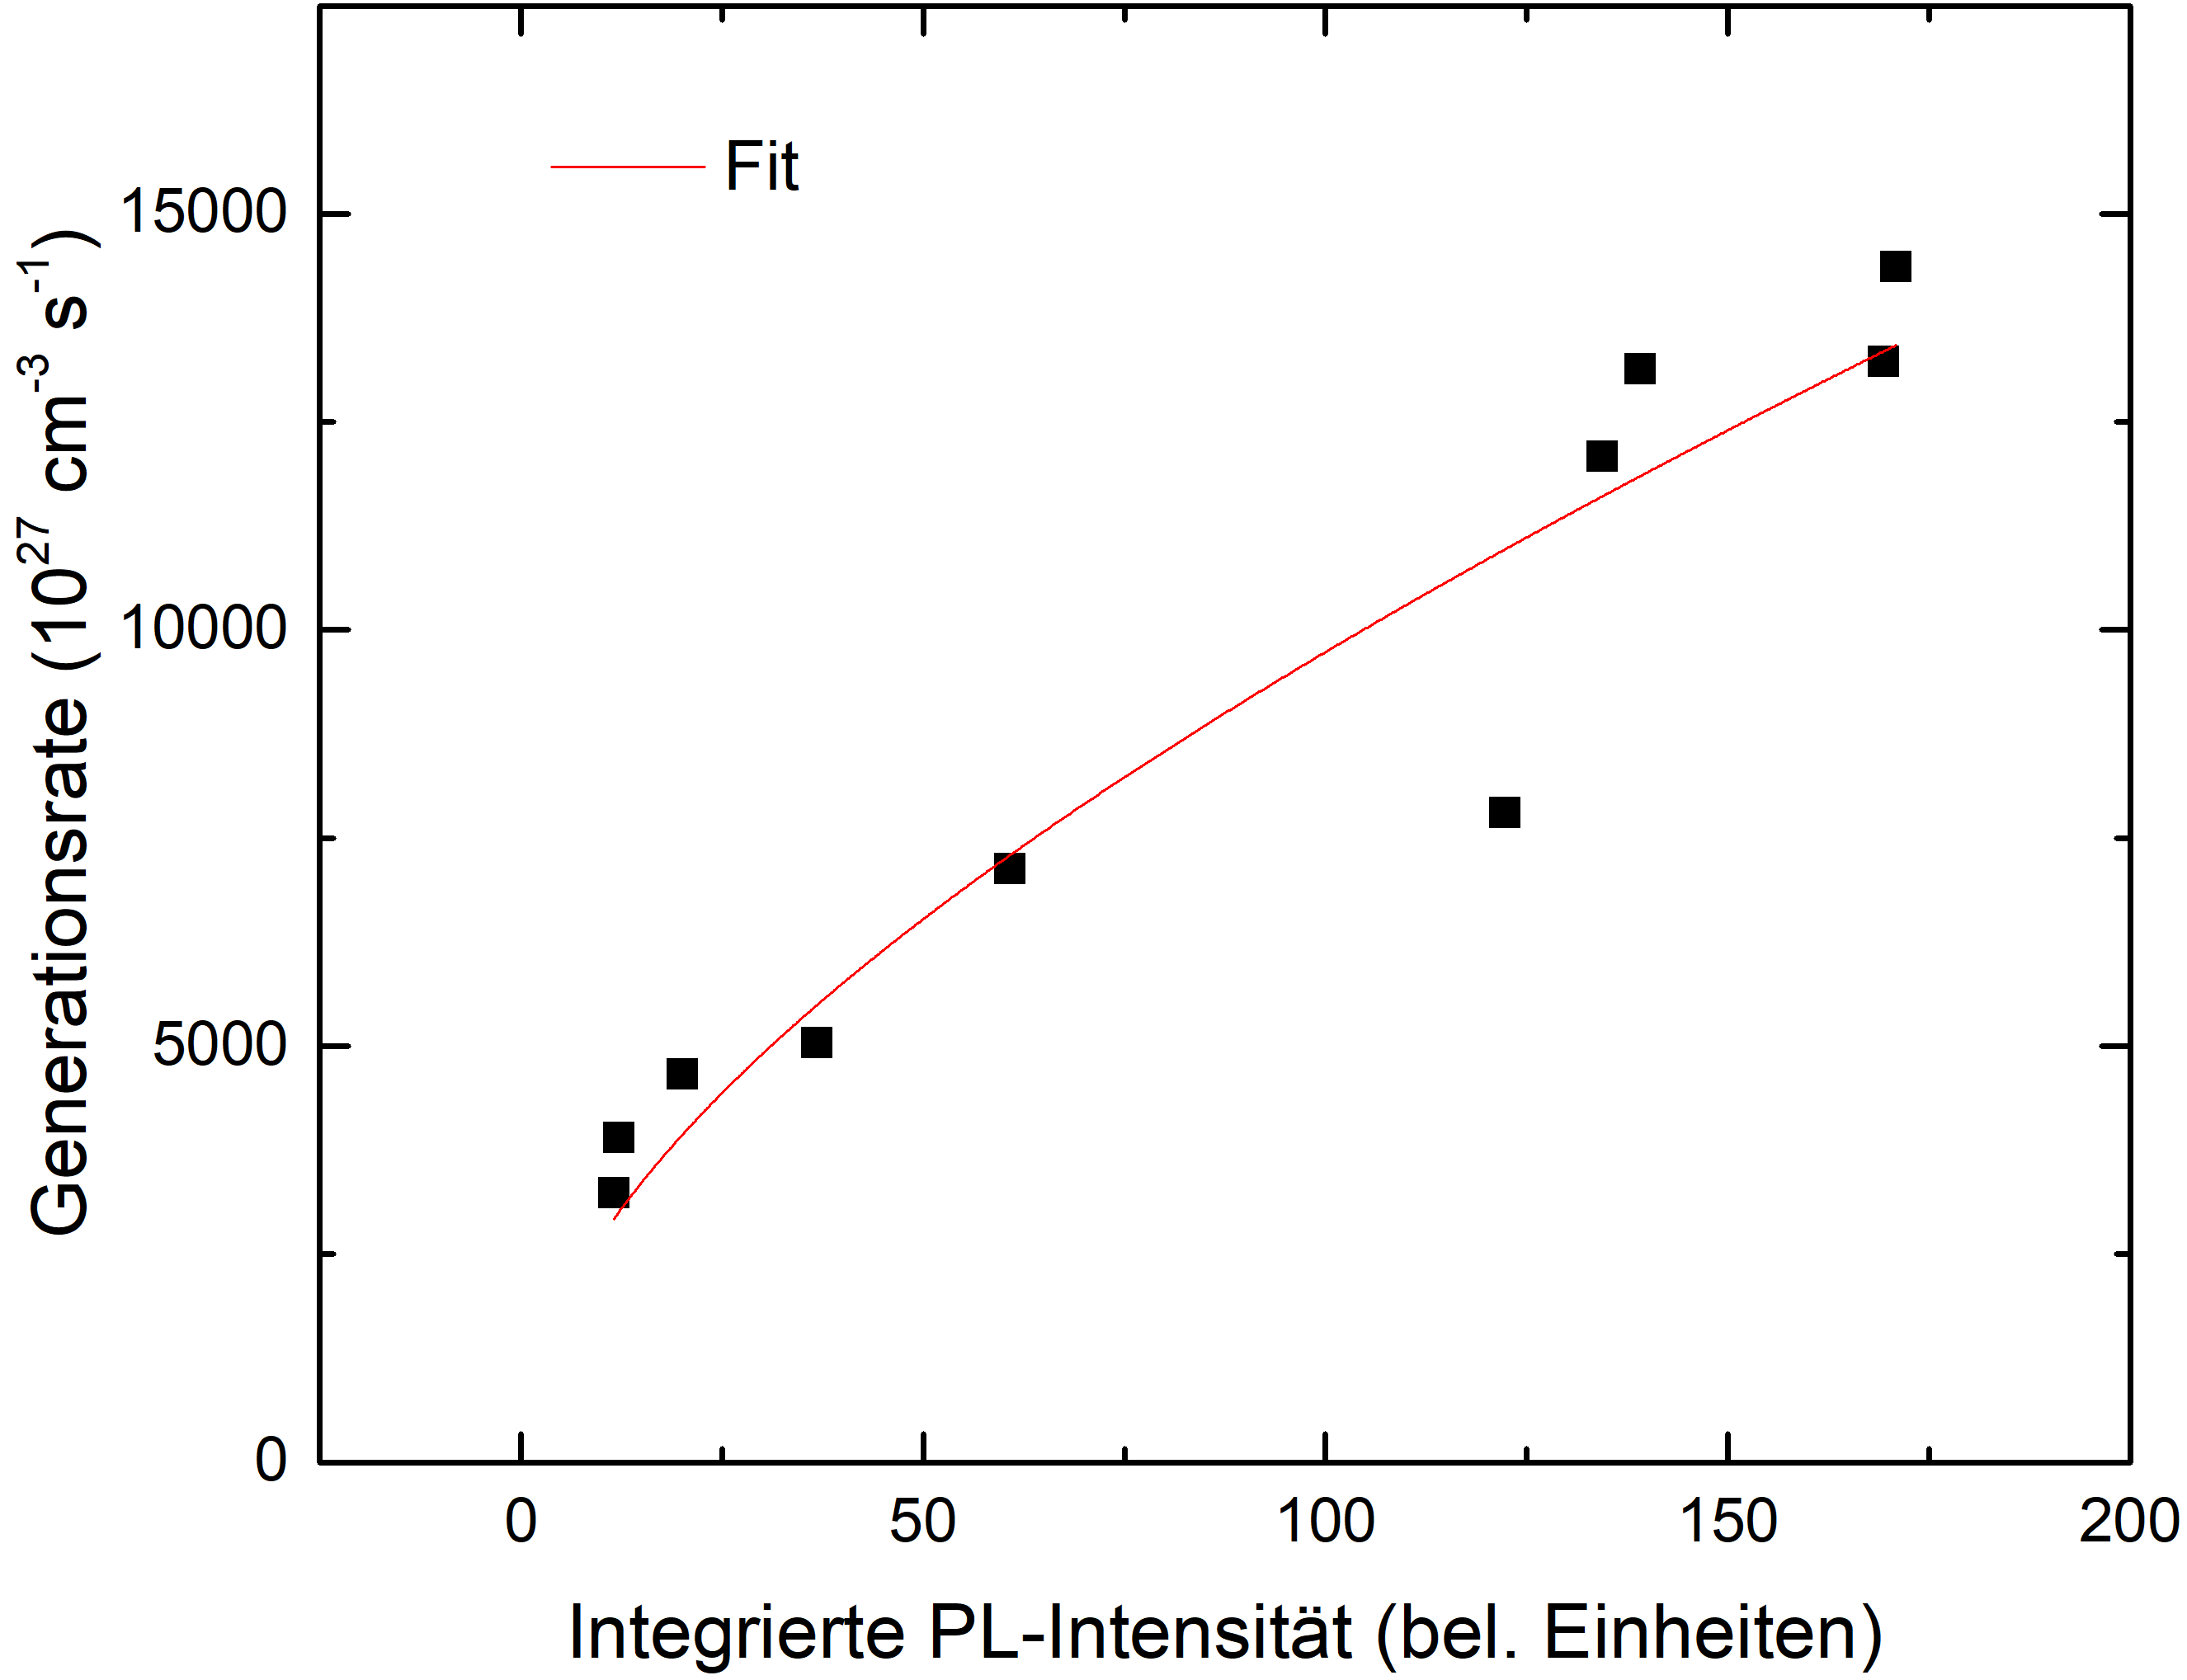
\includegraphics[width=0.30\textwidth]{Bilder/RaumtempBilder/genfit1-10.png} & 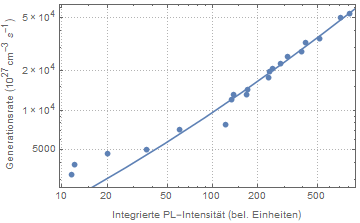
\includegraphics[width=0.30\textwidth]{Bilder/RaumtempBilder/genfit1-20.png}  & 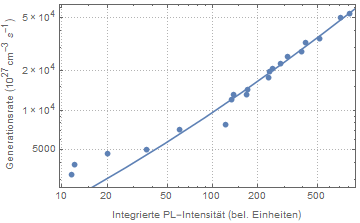
\includegraphics[width=0.30\textwidth]{Bilder/RaumtempBilder/genfit1-20.png} \\
 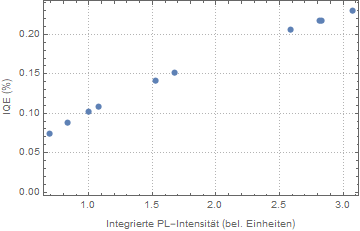
\includegraphics[width=0.30\textwidth]{Bilder/RaumtempBilder/iqe1-10.png} &   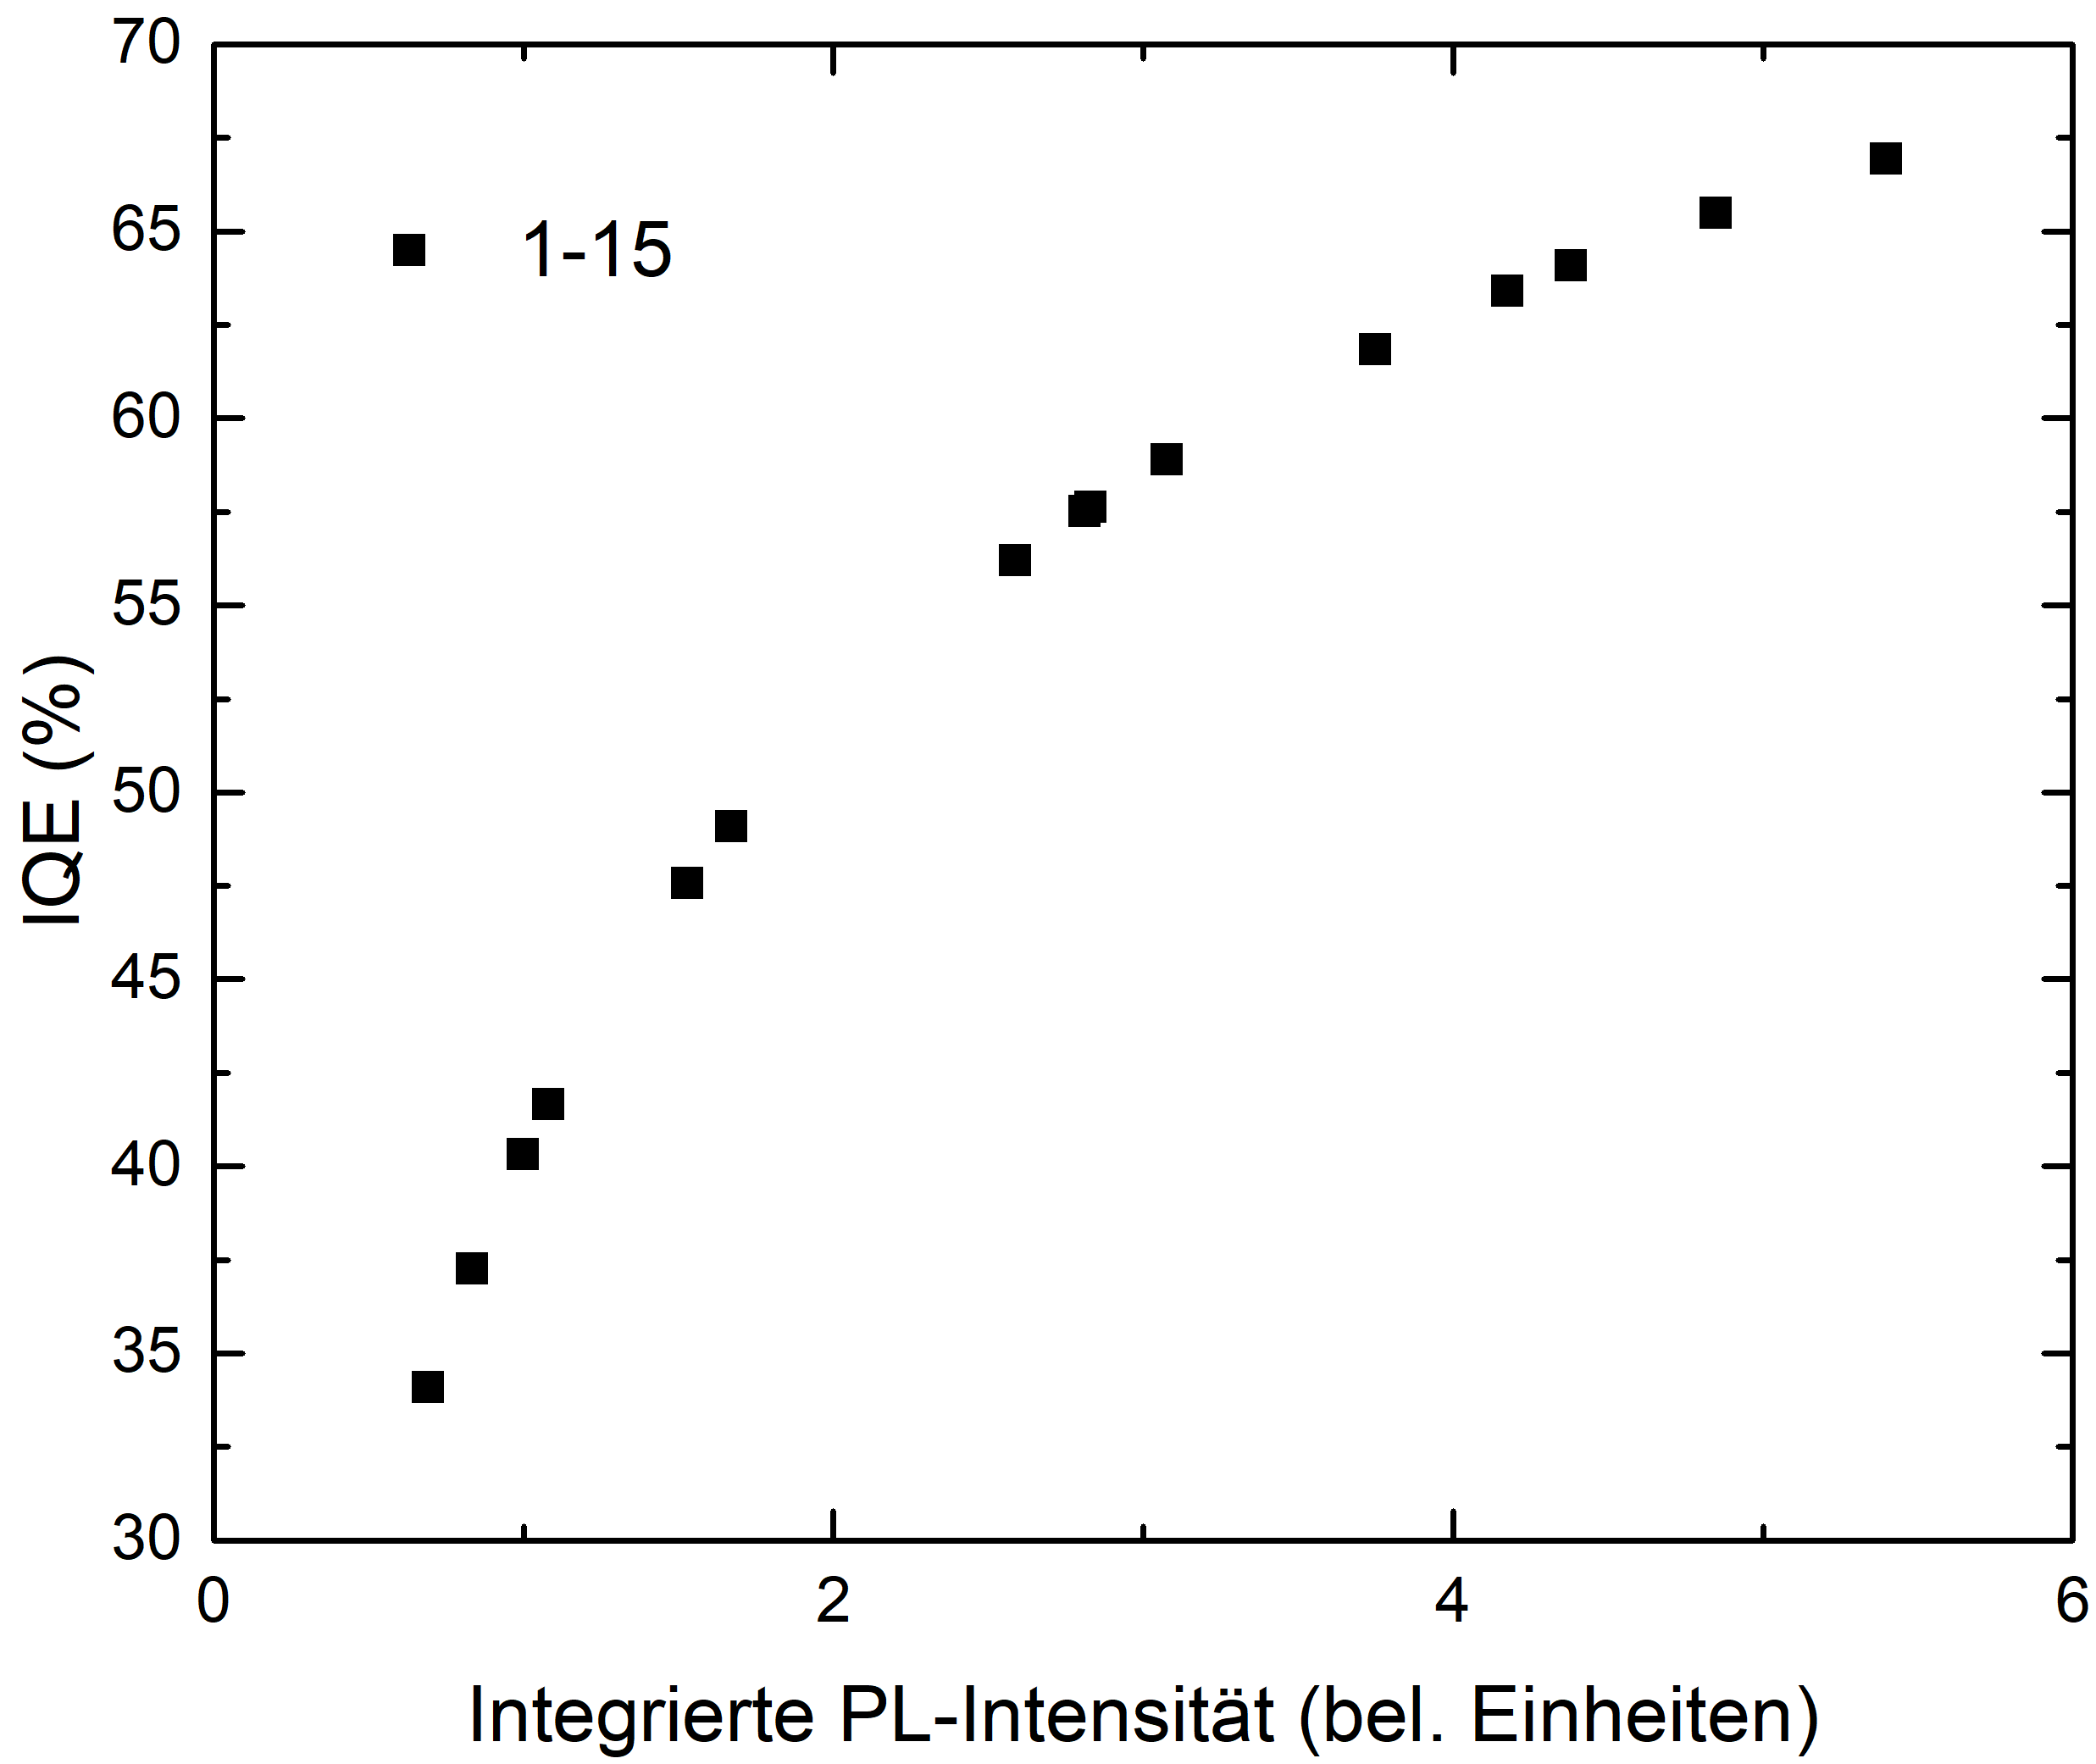
\includegraphics[width=0.30\textwidth]{Bilder/RaumtempBilder/iqe1-15.png} & 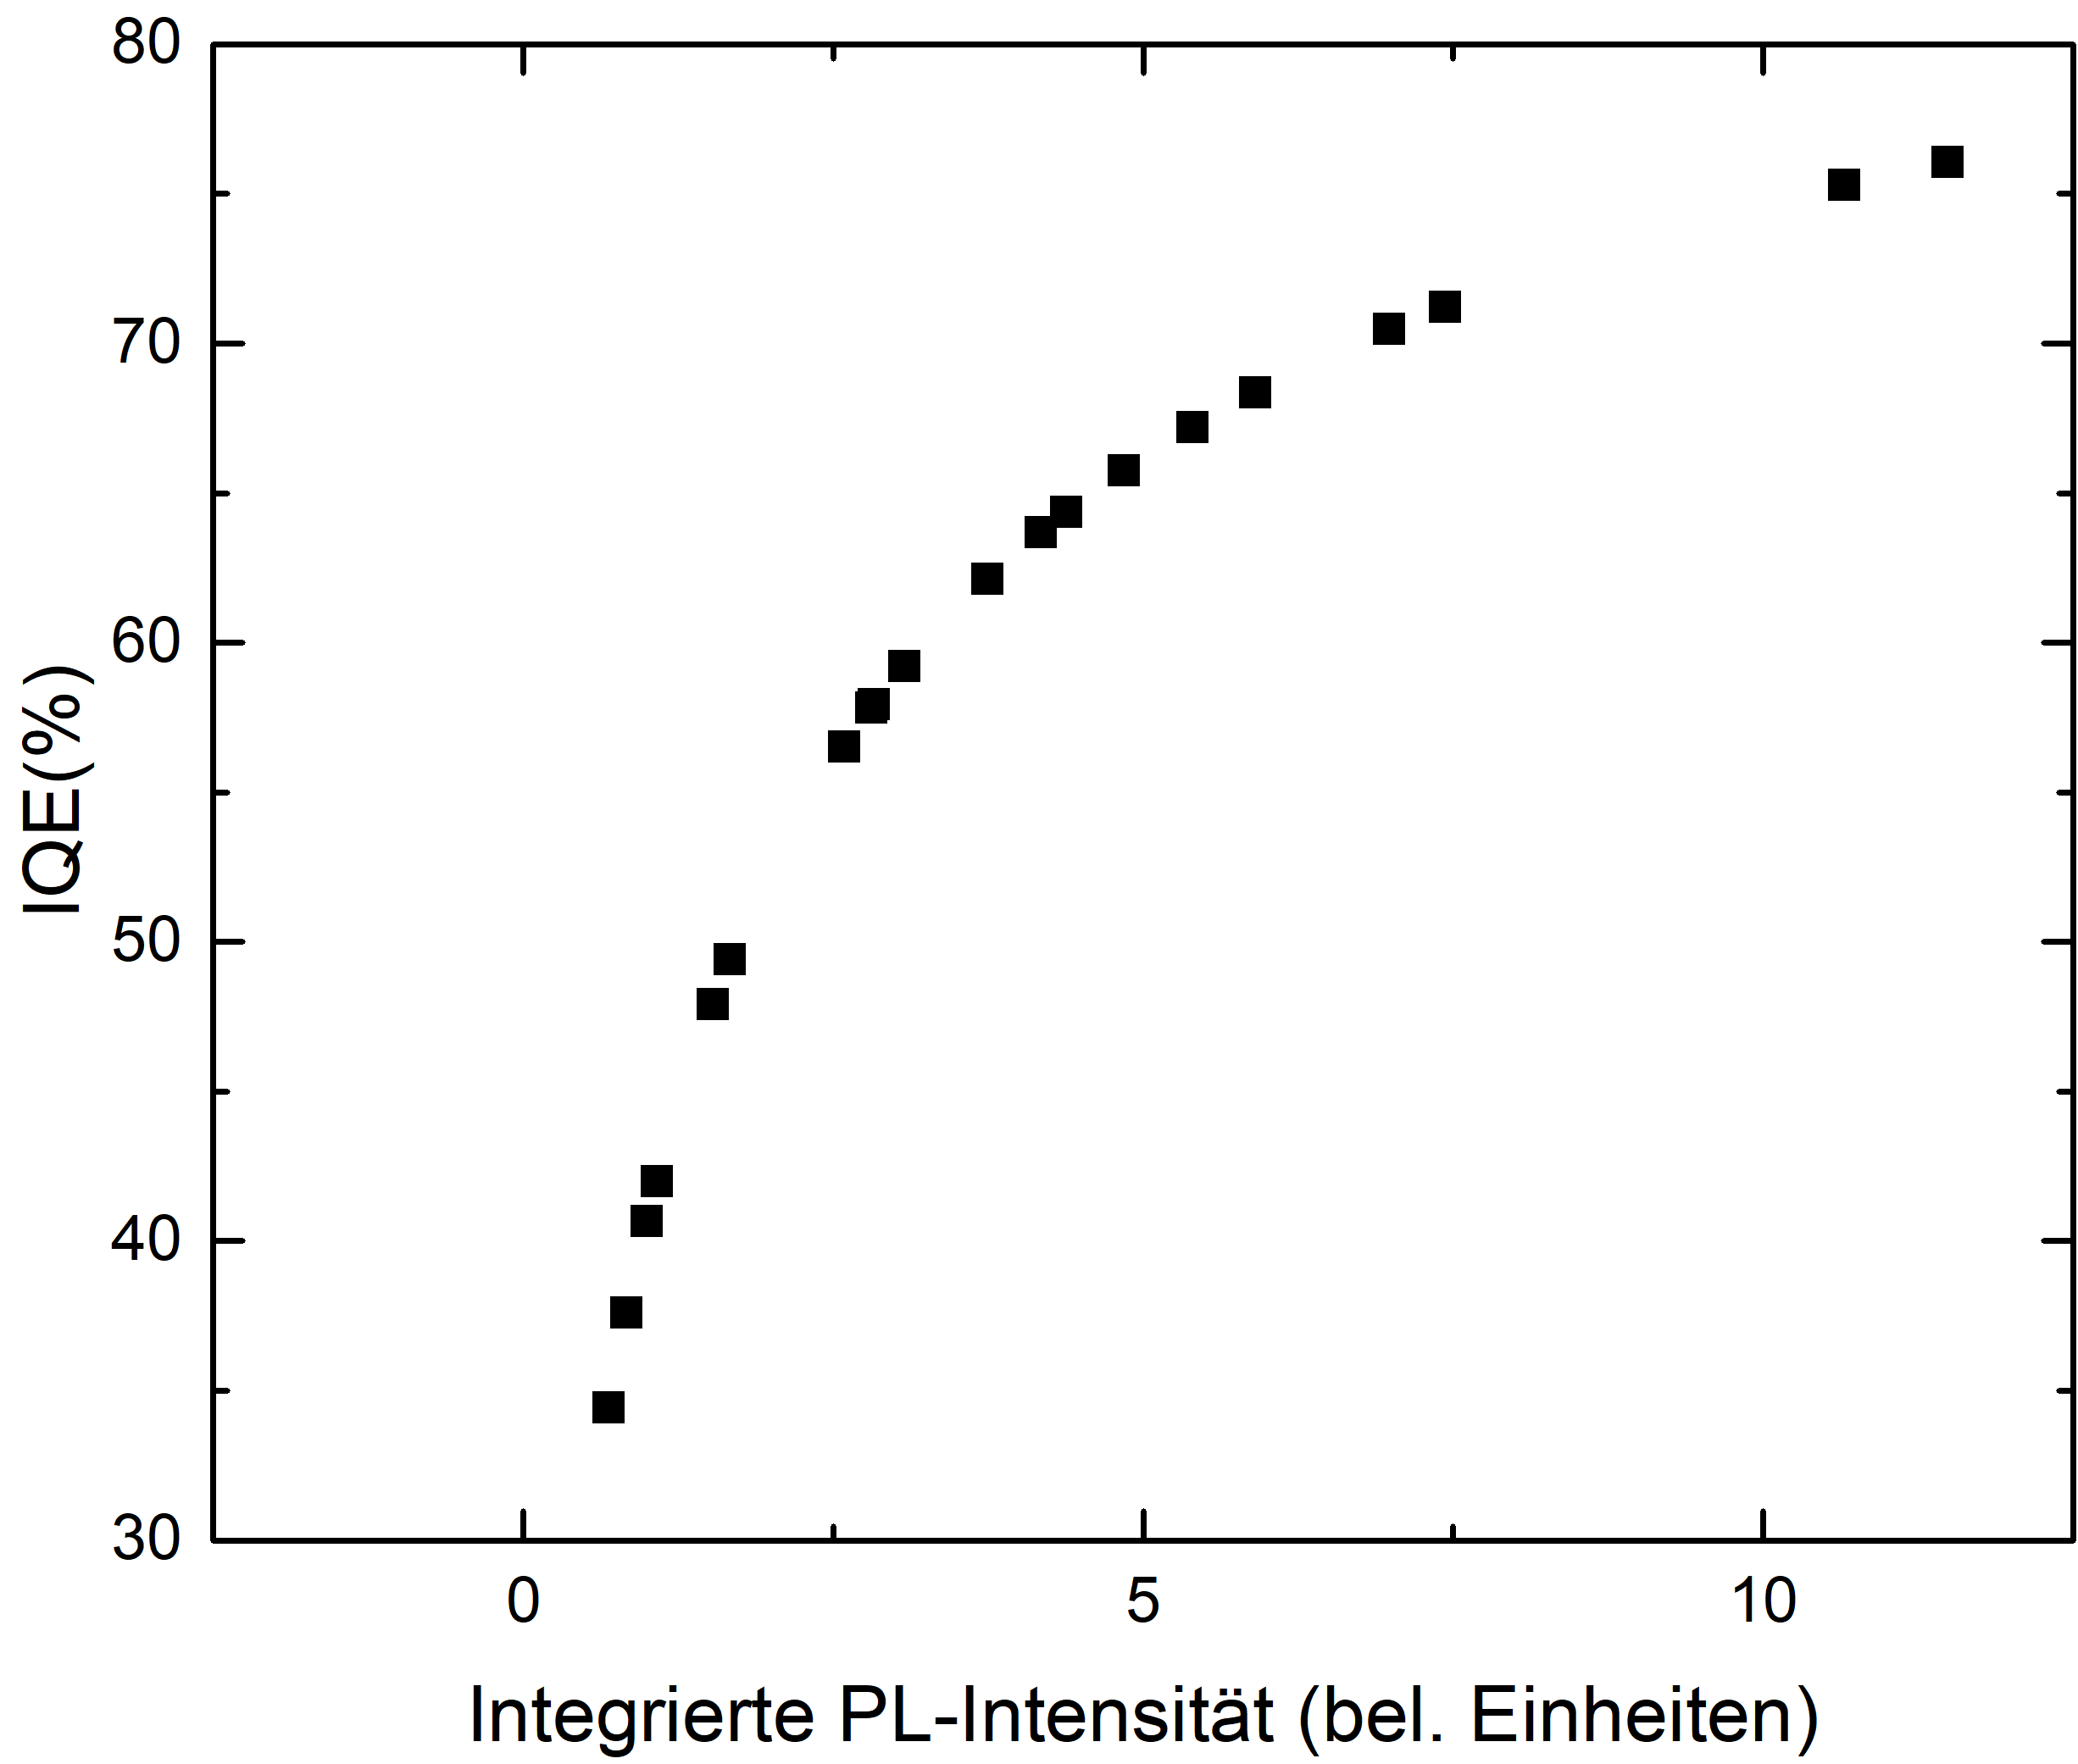
\includegraphics[width=0.30\textwidth]{Bilder/RaumtempBilder/iqe1-20.png}  \\
 a & b & c
\end{tabular}
\caption{Der Fit der Generationsrate in Abhängigkeit der integrierten Intensität für die 1-5 (a), 1-10 (b) und 1-15 (c) Datenpunkte und darunter die aus dem Fit bestimmte IQE.}
\label{fig:raumtemp}
\end{figure}
\noindent 
Angewendet ergab sich, dass die Methode für keine Probenserie verlässliche Werte lieferte für die IQE lieferte und stattdessen die Ergebnisse stark mit dem ausgewählten Bereich der Datenpunkte variierten. Die große Schwankung in Abhängigkeit der ausgewählten Datenpunkte ist in Abbildung \ref{fig:raumtemp} zu sehen.
\newline
Dieses Verhalten mit der starken Schwankung wiesen alle untersuchten Proben auf. 
Des Weiteren sollte erwähnt werden, dass die zugehörigen A- und B-Parameter in keinem der Fälle in einem Bereich lagen, in dem sie nach Literaturwerten einzuordnen wären. Stattdessen schwankten sie variierend mit einigen Zehnerpotenzen darüber oder darunter. 
\newline
Nun soll auf einige Probleme des Ansatzes der angewandten Methode eingegangen werden. 
Die Methode setzt voraus, dass die Auger-Rekombination vernachlässigt werden kann, da nur Bereiche geringer Anregungsleistungsdichte betrachtet werden sollten. Dieser Bereich leidet aber insbesondere bei Raumtemperatur an starkem Rauschen. 
\newline
Zusätzlich betrachtet die Methode den möglichen Einfluss einer Dotierung überhaupt nicht. Dies ist nicht zu vernachlässigen wie in Kapitel \ref{chap:grundfitting} beschrieben und gezeigt.
\newline
Einer weiterer wichtiger Punkt ist, dass mit dem von uns genutzten Setup keine Möglichkeit bestand, nur die QWs anzuregen und so den Effekten thermischer Diffusion ebenfalls nicht Rechnung getragen wird. 
\newline
Als Fazit bleibt nur zu sagen, dass die Methode für die Bestimmung der IQE unserer Proben als nicht anwendbar beschrieben werden muss.
%Bei Proben mit Laserstruktur (erste und letzte Barriere des MQWs sind Waveguides) fiel insbesondere auf, dass die Form der Kurve von der des Fits besonders stark abweicht und wahrscheinlich bedingt ist, durch die komplexere Struktur im Vergleich zu normalen LED-Strukturen. 

